\documentclass[11pt,a4paper]{report}
\usepackage[portuges]{babel}
\usepackage[utf8]{inputenc}
\usepackage{graphicx}
\usepackage{url}
\usepackage{enumerate} 
\usepackage{lmodern}

%\usepackage{apalike} % gerar biliografia no estilo 'named' (apalike)

\usepackage{color}
\usepackage{multirow} 
\usepackage{array} 
\usepackage[pdftex]{hyperref}
\usepackage[font=small,labelfont=bf]{caption}


\definecolor{saddlebrown}{rgb}{0.55, 0.27, 0.07}

\usepackage{listings}  % para utilizar blocos de texto verbatim no estilo 'listings'
%paramerização mais vulgar dos blocos LISTING - GENERAL
\lstset{
	basicstyle=\small, %o tamanho das fontes que são usadas para o código
	numbers=left, % onde colocar a numeração da linha
	numberstyle=\tiny, %o tamanho das fontes que são usadas para a numeração da linha
	numbersep=5pt, %distancia entre a numeração da linha e o codigo
	breaklines=true, %define quebra automática de linha
    frame=tB,  % caixa a volta do codigo
	mathescape=true, %habilita o modo matemático
	escapeinside={(*@}{@*)} % se escrever isto  aceita tudo o que esta dentro das marcas e nao altera
}
%
\lstset{ 
	language=Python}							% choose the language of the code
%	basicstyle=\ttfamily\footnotesize,		% the size of the fonts that are used for the code
%	keywordstyle=\bfseries,					% set the keyword style
%	%numbers=left,							% where to put the line-numbers
%	numberstyle=\scriptsize,				% the size of the fonts that are used for the line-numbers
%	stepnumber=2,							% the step between two line-numbers. If it's 1 each line
%											% will be numbered
%	numbersep=5pt,							% how far the line-numbers are from the code
%	backgroundcolor=\color{white},			% choose the background color. You must add \usepackage{color}
%	showspaces=false,						% show spaces adding particular underscores
%	showstringspaces=false,					% underline spaces within strings
%	showtabs=false,							% show tabs within strings adding particular underscores
%	frame=none,								% adds a frame around the code
%	%abovecaptionskip=-.8em,
%	%belowcaptionskip=.7em,
%	tabsize=2,								% sets default tabsize to 2 spaces
%	captionpos=b,							% sets the caption-position to bottom
%	breaklines=true,						% sets automatic line breaking
%	breakatwhitespace=false,				% sets if automatic breaks should only happen at whitespace
%	title=\lstname,							% show the filename of files included with \lstinputlisting;
%											% also try caption instead of title
%	escapeinside={\%*}{*)},					% if you want to add a comment within your code
%	morekeywords={*,...}					% if you want to add more keywords to the set
%}

\usepackage{xspace}

\parindent=0pt %espaço a deixar para fazer a  indentação da primeira linha após um parágrafo
\parskip=2pt % espaço entre o parágrafo e o texto anterior

\setlength{\oddsidemargin}{-1cm} %espaço entre o texto e a margem
\setlength{\textwidth}{18cm} %Comprimento do texto na pagina
\setlength{\headsep}{-1cm} %espaço entre o texto e o cabeçalho
\setlength{\textheight}{23cm} %altura do texto na pagina

% comando '\def' usado para definir abreviatura (macros)
% o primeiro argumento é o nome do novo comando e o segundo entre chavetas é o texto original, ou sequência de controle, para que expande
\def\darius{\textsf{Darius}\xspace}
\def\antlr{\texttt{AnTLR}\xspace}
\def\pe{\emph{Publicação Eletrónica}\xspace}
\def\titulo#1{\section{#1}}    %no corpo do documento usa-se na forma '\titulo{MEU TITULO}'
\def\super#1{{\em Supervisor: #1}\\ }
\def\area#1{{\em \'{A}rea: #1}\\[0.2cm]}
\def\resumo{\underline{Resumo}:\\ }

%\input{LPgeneralDefintions} %permite ler de um ficheiro de texto externo mais definições



\title{

\begin{center}

\includegraphics[scale=0.3]{images/um}
\end{center}

Processamento de Linguagens \\
		3º ano de MIEI\\  \vspace{1cm}
       \textbf{Trabalho Prático 1\\ 
			Problema nº2}\\  \vspace{1cm} Relatório de Desenvolvimento \\
      ER + Filtros de Texto \\ \vspace{2cm}
\large{Grupo 46}}

\author{ Ana Filipa Pereira\\ (A89589) \and Carolina Santejo\\ (A89500)
         \and Raquel Costa\\ (A89464)
       }

\date{\vspace{2cm}\today} 

\begin{document}


\maketitle % apresentar titulo, autor e data




\begin{abstract}  % resumo do documento
	\qquad Este primeiro trabalho realizado no âmbito da cadeira de Processamento de liguagens consistiu na criação de um projeto em \textit{Python} capaz de filtrar informação de um ficheiro XML e assim responder às várias alíneas pedidas. De acordo com o método de seleção do exercício, o grupo ficou com o problema número 2, sendo este relativo ao registo de rapazes que pretendiam seguir a vida clerical e que se candidatavam aos seminários.\par
	\qquad Neste relatório está explicado detalhamente todos os passos da resolução de cada alíneas,nomeadamente o raciocínio por de trás da solução proposta e a justificação das Expressões Regulares utilizadas.\par
	\qquad Este projeto teve como principais objetivos a consolidação dos conhecimentos adquiridos ao longo das auas teóricas e práticas, nomeadamente a familiarização  com o módulo RE do \textit{Python}, a capacidade de escrever Expressões Regulares para descrição de padrões de frases dentro de textos, e o desenvolvimento , a partir de ERs, de Filtros de Texto ou Processadores de Linguagens Regulares que filtrem textos com base no conceito de regras de produção Condição-Ação.
\end{abstract}



\tableofcontents 

\listoffigures 




\chapter{Introdução} \label{chap:intro} 			%  -------------------------------------- INTRODUÇÃO --------------------------------------------


\section{Enquadramento e Contexto}
\area{Processamento de Linguagens}


	\qquad O ficheiro XML fornecido para a resolução deste problema, contêm milhares de processos de indivíduos candidatos ao seminário, sendo que cada processo possui o \textit{id} respetivo, o número da pasta , a data de candidatura, o nome do candidato, o nome da sua mãe e do seu pai (caso fosse conhecido) e o nome e grau de parentesco de familiares que também se candidataram ao seminário.\par
	\qquad O objetivo deste projeto, consistiu, então, na extração da informação deste ficheiro XML, sendo esta posteriormente organizada e tratada de forma a responder às várias alíneas do problema inicial.


\section{Problema e Objetivo}

	\qquad Numa primeira fase, foi necessário analisar a estrutura do ficheiro XML e tentar perceber a informação que ele possuia. Após isto, e tendo sido detetados padrões no texto, seguiu-se a escolha das Expressões Regulares a utilizar, tendo em conta o que era pedido para cada alínea.\par
	\qquad Posteriormente, foi essencial definir como é que a informação que ia sendo obtida do ficheiro seria guardada temporariamente. Após isto, a informação lida é tratada e organizada de maneira a apresentá-la, de forma intuitiva e agradável, ao utilizador.


\section{Decisões tomadas}

	\qquad Tal como referido, para o desenvolvimento deste trabalho prático foi utilizada a linguagem de programação \textit{Python}. Trata-te de uma linguagem flexível, pois não existem regras rígidas sobre como criar recursos, e, como tal, existem diversos métodos para construir uma solução. Sendo assim, uma vez que o objetivo deste trabalho é aprodundar e aplicar o conhecimento do grupo no que toca a Expressões Regulares e Filtos de Texto, foi decidido que iríamos tirar o máximo partido das mesmas, chegando a várias soluções diferentes para o mesmo problema, tanto utilizando diferentes estratégias de \textit{Python}, como diferentes ER's.



\section{Estrutura do Relatório}

	  \qquad Este relatório possui 5 capítulos. \par
	  \qquad No capítulo 1, Introdução, é feito o enquadramento e contextualização do projeto, bem como uma breve descrição do problema em mãos. É feita também, uma referência às decisões tomadas no trabalho.\par
	  \qquad No capítulo 2, Análise  e Especificação, é feita uma descrição informal do desafio em questão, além de serem especificados os requisitos necessários. Neste capítulo, fala-se também da forma como os dados são lidos e guardados temporariamente.\par
	 \qquad  No capítulo 3, Implementação, é explicado , detalhadamente, a resolução de cada alínea nomeadamente as Expressões Regulares utilizadas. Em certas alíneas o grupo adicionou funcionalidades extras, sendo estas também explicadas.\par
	  \qquad No capítulo 4, Codificação e Testes, são apresentados testes realizados e os resultados obtidos.\par
	  \qquad No capítulo 5, Conclusão, é feita uma análise geral do projeto.\par



\chapter{Análise e Especificação} \label{chap:analiseEspecificacao}		% ----------------------- Análise e Especificação ----------------------------------


\section{Descrição informal do problema} \label{sec:descricaoProblema} 

	\qquad O problema em questão consiste no seguinte: dado um ficheiro XML, que possui milhares de processos relativos a cadidaturas ao seminário, é preciso extrair a informação necessária para responder a cada alínea. Para tal é fundamental analisar a estrutura do \textit{dataset} e escolher as ERs mais adequadas para obter os dados desejados.\par
	\qquad A informação obtida tem de ser tratada e apresentada de forma organizada ao utilizador.


\section{Especificação do Requisitos}
	
	Para responder devidamente ao problema proposto, foi necessário apresentar uma solução que cumprisse os seguintes requisitos:\\
	\begin{itemize}
		\item Determinar número de processos por ano,ordenados cronologicamente.
		\item Determinar intervalo de datas dos quais existem registos.
		\item Determinar a frequência de nomes próprios e apelidos a nível global e os 5 mais frequentes em cada século.
		\item Determinar número de candidatos com familiares que também são candidatos.
		\item Determinar grau de parentesco mais comum.
		\item Verificar se a mesma mãe e o mesmo pai têm mais do que um filho candidato ao seminário.
		\item Apresentar todas as árvores geneológicas para um dado ano.
		
	\end{itemize}




\chapter{Concepção/Desenho da Resolução}			% --------------------------------- Concepção/desenho da Resolução ---------------------------------


\section{Leitura dos Dados e Armazenamento}

	\qquad Para armazenar temporariamente a informação lida do ficheiro foi necessário guardá-la em memória.\par 
	\qquad Tendo em consideração a flexibilidade característica da linguagem \textit{Python}, o grupo não sentiu a necessidade de criar novas estruturas de dados. Mas salientamos que caso este projeto fosse desenvolvido numa linguagem como o \textit{C/C++}, então nesse caso a criação de uma \textit{struct} seria fundamental para gerir tantos dados de um ficheiro \textit{XML} tão extenso como este. Além disso, como os ficheiros \textit{XML} seguem por vezes uma estrutura hierárquica e apresentam um padrão específico, seria bastante benéfico a construção de uma estrutura de dados própria para o armazenamento de dados. Mas como temos a possibilidade de utilizar uma linguagem como o \textit{Python}, existem inúmeras soluções às quais podemos chegar através de diversos métodos e recursos, sem esquecer a utilização fulcral de Expressões Regulares. Assim sendo, ao longo da resolução de todos os exercícios foram utilizados tipos de dados simples como listas e tuplos como uma forma de aproveitar ao máximo as funcionalidades das expressões regulares, como por exemplo os grupos.
	



\section{Implementação}

	\section*{Ficheiro a)}

	\textbf{Objetivo:} Calcular o número de processos por ano; Apresentar a listagem por ordem cronológica e indicar o
intervalo de datas em que há registos bem como o número de séculos analisados.
\vspace{0.5cm}

	\qquad Para resolver os vários objetivos da primeira alínea foi necessário obter a data presente em cada processo. Assim, e visto que o ficheiro \textit{XML} é lido linha a linha, utiliza-se a função \textit{search} do módulo \textit{re} para encontrar a primeira ocorrência de uma data em cada linha lida. É de realçar que quando uma data é encontrada este é sempre referente a um processo. 
\vspace{0.7cm}
	\begin{itemize}
	\item \textbf{Expressões Regulares:}
	\end{itemize}
	\qquad A escolha da ER, foi feita tendo em conta que as datas apareciam, no ficheiro da seguinte maneira: \textless data\textgreater AAAA-MM-DD\textless/data\textgreater. Tivemos em consideração que o ficheiro poderia apresentar anos com apenas 3 dígitos, como o ficheiro é bastante extenso, achamos necessário incluir também este caso. Em relação aos meses e aos dias, verificamos que as datas apresentavam sempre dois dígitos para a sua representação.\par
	\qquad Desta forma, a ER usada foi a seguinte: 
	   
	\begin{verbatim}
	    <data>((((\d)|(\d){2})\d{2})(-\d{2}){2})</data>
	 \end{verbatim}                 
                          
       \qquad Esta ER, permite ter 3 \textit{groups}: o group(1) seleciona todos os caracteres que se encontram entre \textless data\textgreater e \textless/data\textgreater, o group(2) seleciona apenas os caracteres referentes ao ano na data em questão, e o group(3) seleciona os caracteres que são os dois primeiros dígitos desse ano.\par
       \qquad Com isto, cada vez que se encontrar uma data no texto esta é adicionada à lista chamada \textit{listaDatas} e o ano desta data é adicionado à lista \textit{listaAnos}. No que diz respeito ao século o que acontece é o seguinte: numa data com 4 dígitos, o número formado pelos dois primeiros dígitos somados com 1, é o século dessa data. Por exemplo, o ano 1780, é o século 18 (17 + 1). Assim, quando uma data é lida, faz-se um cast do group(3) para inteiro, soma-se uma unidade e adiciona-se este valor à lista chamada \textit{listaSeculos}.\par
       \qquad Após as 3 listas estarem preenchidas podemos resolver a alínea.\par 
       \qquad Ora, para obtermos o intervalo de datas das quais há registo, bastou fazer sort da \textit{listaDatas} para organizar as datas cronologicamente e depois obter o primeiro e último elemento dessa mesma lista.\par
       \qquad Para determinarmos o número de séculos analisados, bastou aplicar um \textit{Counter} à lista com os séculos, ou seja, \textit{Counter(listaSeculos)}, sendo que isto devolve uma lista de tuplos em que a \textit{key} é o século e o \textit{value} é o número de vezes que esse século aparece em \textit{listaSeculos}. Assim, contando o número de \textit{keys} obtemos o número de séculos analisados.\par
       \qquad Por último, para calcular o número de processos por ano, o grupo usou um \textit{Counter} em \textit{listaAnos}, seguido de um \textit{sorted}, ou seja, \textit{sorted(Counter(listaAnos).items()}, sendo que o \textit{Counter} cria uma lista de tuplos em que a \textit{key} é o ano e o \textit{value} é o número de vezes que esse ano aparece em \textit{listaAnos}, e o \textit{sorted} ordena os tuplos pela \textit{key}. Assim, visto que cada ano advém de uma data que por sua vez é referente a um processo lido, podemos concluir que o número de vezes que um ano aparece em \textit{listaAnos} é o número de processos desse mesmo ano.

	\vspace{0.5cm}
      	\begin{itemize}
		\item \textbf{Extras}\par

 \qquad Durante a realização desta alínea, o grupo foi encontrando maneiras alternativas de resolver os desafios que iam surgindo.\par
	    \qquad Quando era feita a leitura de uma data de um processo, em vez de a adicionar a listas como foi explicado no tópico acima, poder-se-ia ter feito da seguinte forma: utilizar a função \textit{split} do módulo \textit{re} para obter uma lista com 3 elementos (\textit{resData}), que são o ano, mês e dia, respetivamente, da data em questão. Após isto, e tendo previamente definido duas variáveis globais, \textit{min} e \textit{max},que são inicializadas como listas vazias, compara-se \textit{resData} com a data mínima e máxima. Se for uma data mais antiga, subtitui \textit{min}, se for mais recente, subtitui \textit{max}. Esta forma, é mais trabalhosa, no entanto permite utilizar expressões regulares.\par
	   \qquad  Outra metodologia utilizada, foi para o cálculo dos séculos, mas sem recorrer às \textit{ER}. Em vez de termos uma lista própria para os guardar (\textit{listaSeculo}) utiliza-se a lista dos anos, e aplica-se um \textit{Counter},(\textit{Counter(listaAnos)}), onde cada chave será o ano. Assim,percorre-se todos os anos da lista e calcula-se o século de cada um com a seguinte fórmula:\par
	      \begin{center}
	      	\begin{verbatim}
	      	século = (int(x)/100)+1
	      \end{verbatim}
	      \end{center}
     \qquad  Após isto, adiciona-se o século obtido a uma lista própria para o efeito.
	\end{itemize}

	\newpage
	\section*{Ficheiro b)}

	\textbf{Objetivo:} Calcular a frequência de nomes próprios e apelidos global e mostrar os 5 mais frequentes em cada século.
	\begin{itemize}
	\item \textbf{Expressões Regulares}
	\end{itemize}
	
	\begin{enumerate}
		\item \begin{verbatim} r'<nome>(([A-Z][a-z]+) ([A-Z][a-z]+ )*([A-Z][a-z]+))</nome>'  \end{verbatim} 
		\item \begin{verbatim} r'<data>((((\d)|(\d){2})\d{2})-.+)</data>  \end{verbatim} 
	\end{enumerate}	
	
	\qquad Para resolver esta questão, foi utilizada, em primeiro lugar a ER 1 para capturar cada nome completo encontrado. Utilizando os grupos foi possível separar os nomes próprios (group(2)) dos ultimos nomes (group(4)). Cada vez que um nome era encontrado, era procurada a data do mesmo processo utilizando a ER 2, filtrado o seu século (group(3)+1) e colocado nas listas correspondentes os tuplos (nome proprio, seculo) e  (ultimo nome, seculo).
Depois de ter todo o ficheiro percorrido, foram utilizadas as bibliotecas Counter, itemgetter e groupby para agrupar os nomes por seculo e contar o número de ocorrencias de cada um.


	\begin{itemize}
		\item \textbf{Extras}
	\end{itemize}

	\qquad Para capturar o nome presente no processo de cada candidato, foram construídas várias expressões regulares. De todas destacamos duas, a que foi apresentada anteriormente e a seguinte:
	   \begin{verbatim}
			 r'<nome>([a-zA-Z]+)[a-zA-Z ]* ([a-zA-Z]+)</nome>'  
	   \end{verbatim} 
	\qquad A diferença entre esta e a anterior, é que esta consegue capturar nomes que não tenham a primeira letra como maiúscula, aliás consegue capturar nomes dos quais as letras estejam tanto em minúscula como em maiúscula. Decidimos aplicar a outra expressão regular apresentada, uma vez que no ficheiro \textit{XML} o padrão apresentado é que todos os nomes começam por maiúscula, sendo as restantes letras apresentadas em minúscula.
	
\vspace{1cm}
	\section*{Ficheiro c)}

	\textbf{Objetivo:} Calcular o número de candidatos que têm parentes (irmão, tio, ou primo) eclesiásticos; E qual o tipo de parentesco mais frequente.\par
	\vspace{0.5cm}
	\qquad Para a resolução desta alínea, tivemos de dispensar o método da leitura de linha a linha, uma vez que iremos ter de analisar o campo \textless obs\textgreater de cada processo, e como poder ter mais do que uma linha, temos de conseguir capturar o campo inteiro desde \textless obs\textgreater até \textless /obs\textgreater .

	\begin{itemize}
		\item \textbf{Expressões Regulares}
		 \begin{enumerate}
		\item \begin{verbatim} r'(<obs>(\n|.)*?</obs>)'  \end{verbatim} 
		\item \begin{verbatim} r'(Irmao|Tio|Primo)'  \end{verbatim} 
	\end{enumerate}

	Primeiro, começamos por usar a ER nº1 , e usamos do \textit{package re} o método \textit{findall}, deste modo iremos obter uma lista com todos os campos \textless obs\textgreater de cada processo. De seguida iremos percorrer esta lista, e iremos verificar se as observações de cada processo contém alguma informação sobre os parentes do candidato. \par
	\qquad Para tal, usamos a segunda ER, e novamente, o método \textit{findall}. Assim sendo, iremos obter uma lista com as correspondências aos parentes "Irmão", "Tio" e "Primo", que, posteriormente, caso não seja vazia iremos percorrer e adicionar a uma lista global que contém os graus de parentesco de cada candidato existente. O resultado final desta lista será algo do tipo:\par
		\begin{verbatim}
			 ['Irmao','Primo','Primo','Tio',.....]  
	   \end{verbatim} 
	\qquad Com base nisto, aplica-se um Counter, que consiste numa subclasse do \textit{package collections}, a esta lista global. O resultado disto será uma lista de tuplos, onde a key é o grau de parentesco e o value é o número de vezes que este grau de parentesco se repete. Após isto, aplica-se o método \textit{most\textunderscore common(1)}, de modo a obter o grau de parentesco mais frequente no ficheiro \textit{XML} analisado.\par
	\qquad Em relação ao cálculo do número de candidatos que têm parentes eclesiásticos, apenas foi colocado um contador que aumenta um valor a cada iteração do ciclo em que é encontrado pelo menos um parente no campo das observações do candidato em análise.
	
		
	\end{itemize}
\vspace{1cm}

	\section*{Ficheiro d)}
	\textbf{Objetivo} Verificar se o mesmo pai ou a mesma mãe têm mais do que um filho candidato.
\vspace{0.5cm}

	\qquad Nesta alínea, decidimos dar a possibilidade do utilizador escolher qual o casal de pais que quer analisar. Para tal ele deve indicar o ID do processo do candidato ( e não o nome, porque existe uma enorme quantidade de nomes repetidos), para conseguir verificar os outros filhos dos seus pais.\par
	\qquad Primeiramente, tal como foi feito na alínea anterior todo o conteúdo ficheiro é lido e armazenado numa variável. De seguida, recorre-se à função \textit{procuraID}, que irá receber como input o id do filho que o utlizador forneceu e um inteiro que poderá tomar o valor de 1 ou 0, para já é dado o valor de 1.\par
	\qquad Esta função tem como objetivo encontrar a mãe e o pai do filho cujo id foi fornecido, que posteriormente, serão adicionados a uma lista global. Após isto são analisados os irmãos do candidato em questão e caso se encontre, voltamos a chamar a função, mas desta vez damos o valor de 0 no seu input, de forma a sinalizar que não são os pais deste cadidato que estamos a verificar, uma vez que um dos pais do irmão pode não ser o pai/mãe do candidato que o utilizador da aplicação indicou. Portanto, iremos analisar os pais deste irmão e caso sejam os mesmos do candidato inicial, então são adicionados à lista global.\par
	\qquad Assim sendo, no final, iremos apenas aplicar um \textit{Counter} à lista global dos pais, resultando numa lista de tuplos cuja key é o nome da mãe ou do pai e o value é o número de vezes que se repetem na lista, ou seja, é o número de filhos de cada um deles.\par

\vspace{0.5cm}

	\begin{itemize}
		\item \textbf{Expressões Regulares}

			 \begin{enumerate}
				\item \begin{verbatim}rf'<processo id="({id})">(\n|.)*?</processo>'  \end{verbatim} 
				\item \begin{verbatim}r'<mae>(([A-Z][a-z]+) ?([A-Z][a-z]+ )*([A-Z][a-z]+)?).*</mae>'  \end{verbatim} 
				\item \begin{verbatim}r'<pai>(([A-Z][a-z]+) ([A-Z][a-z]+ )*([A-Z][a-z]+)).*</pai>'  \end{verbatim} 
				\item \begin{verbatim}r'(Irmao). *Proc.(\d+)'  \end{verbatim} 
			\end{enumerate}

	\qquad A ER nº1 foi utilizada para encontrar o processo cujo ID é aquele indicado pelo utilizador. Depois disto, partimos para a procura da mãe e do pai do candidato desse mesmo processo encontrado através da ER nº2 e da ER nº3. Para encontrar o/os irmão(s) do candidato, foi usada a ER nº4.\par
		
		\item \textbf{Extras}\par
\vspace{0.5cm}
	\qquad Através desta resolução, o utilizador não só consegue ver o nº de filhos de cada pai/mãe de um candidato à sua escolha, como também consegue ver quem são os seus irmãos.\par
	\qquad Além disso, o grupo, de forma a testar o programa e a verificar por mera curiosidade, quais os filhos que têm irmãos de pai ou mãe diferente, decidiu fazer algo extra. Portanto, foi aplicada a resolução construída a todos os processos, analisando assim os pais de cada candidato existente. Desta forma, é possível descobrir quem são os pais e as mães que têm filhos com um parceiro diferente daquele que é registado no processo que está a ser analisado. Para tal, criamos uma lista "traicoes", e no momento em que estamos a analisar os pais do irmão ou dos irmãos de um candidato, concluímos o seguinte: caso a mãe de ambos seja diferente, adicionamos o nome do pai à lista, caso o pai seja diferente adicionamos o nome da mãe.\par
	\qquad Desta forma, foi possível testar a resolução e corrigir problemas de implementação, verificamos também que estar a percorrer os processos todos para analisar os pais registados em cada processo, trata-se de um método bastante lento e demorado. Mas como o objetivo é analisar os pais de um só processo, concluímos então que trata-se de um promenor que não é prejudicial.

	\end{itemize}

\vspace{1cm}

	\section*{Ficheiro e)}

	\textbf{Objetivo} Utilizando a linguagem de desenho de grafos DOT desenhe todas as árvores genealógicas (com
	base nos triplos $<$filho, pai, mãe$>$) dos candidatos referentes a um ano dado pelo utilizador.\par
	
	\begin{itemize}
	\item \textbf{Expressões Regulares}
	\end{itemize}
	

	\begin{enumerate}
	\item  \begin{verbatim} rf'(<processo id="(\d+)">\n *<pasta>\d+</pasta>\n *<data>({ano})-.+(\n|.)*?</processo>)'  \end{verbatim} 
	\item  \begin{verbatim} r'<nome>(([A-Z][a-z]+) ?([A-Z][a-z]+ )*([A-Z][a-z]+)?).*</nome>'  \end{verbatim} 
	\item  \begin{verbatim} r'<mae>(([A-Z][a-z]+) ?([A-Z][a-z]+ )*([A-Z][a-z]+)?).*</mae>'  \end{verbatim} 
	\item  \begin{verbatim} r'<pai>(([A-Z][a-z]+) ([A-Z][a-z]+ )*([A-Z][a-z]+)).*</pai>'  \end{verbatim} 
	\item  \begin{verbatim} r'(Irmao). *Proc.(\d+)'  \end{verbatim} 
	\item  \begin{verbatim} rf'<processo id="({id})">'  \end{verbatim} 
\end{enumerate}

	\qquad Para resolver esta questão, inicialmente foi utilizada a ER 1 para ir buscar todos os processos existentes no ano solicitado. Para cada processo foram filtrados os nomes da pessoa (expressão 2), da sua mãe (ER 3) e do seu pai (ER 4). Para além disso foi necessário verificar se a pessoa em questão tem irmãos logo foi aplicada também a ER 5. Caso tenha, foi necessário aceder novamente à lista de processos para filtrar o nome de cada um (ER 6). Posteriormente cada um dos irmãos é retirado da lista para que não haja árvores repetidas. \par
	\qquad No final são agrupados os nomes de todos os elementos da familia numa lista, posteriormente, essa lista é adicionada à lista global de familias.\par
	\qquad Tendo a lista completa de famílias, percorremos a mesma obtendo ao fim de cada iteração uma sublista com os membros de uma familia, e a partir daí chamamos a função \textit{desenhaFamilias}, onde passamos como input a familia que queremos desenhar. No final do ciclo iremos obter o desenho da árvore genealógica de cada família (sublista) presente na lista global das familias. As árvores genealógicas foram geradas com recurso à biblioteca \textit{graphviz} onde cada nodo pai ou mãe liga aos seus respetivos filhos.\par
	\qquad Além disso, são apresentadas num só ficheiro apresentado em formato \textit{png}.
	
	
\vspace{1cm}

	\section*{Menu}


	    \qquad Durante o planeamento do projeto, o grupo decidiu que seria mais organizado criar um programa para cada uma das 5 alíneas do problema. \par
	    \qquad No entanto, de maneira a que o utilizador tivesse uma experiência mais agradável e intuitiva, foi criado um Menu, cuja função é executar o programa relativo à alínea que o \textit{user} escolher. Na figura seguinte, é apresentada a interface obtida através deste ficheiro.

\vspace{1cm}

\begin{center}
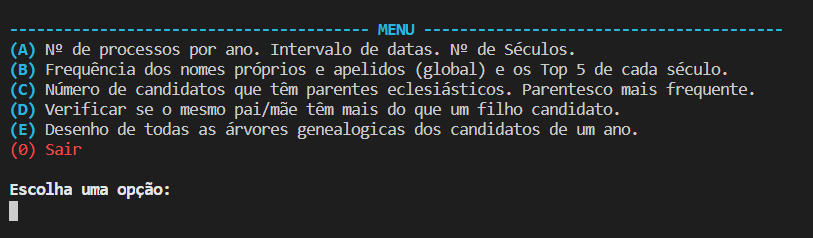
\includegraphics[scale=0.9]{images/menu}
\captionof{figure}{Menu - Interface da aplicação}
\end{center}
	 
	

\chapter{Codificação e Testes}  	% ---------------------------------------------------------- Codificação e Testes ------------------------------------------------------------------------------

\section{Testes realizados e Resultados}

\qquad De seguida encontram-se alguns testes e resultados obtidos pelo grupo no final do desenvolvimento do programa.\par

	\subsection*{ Alínea a)}

	\begin{center}
	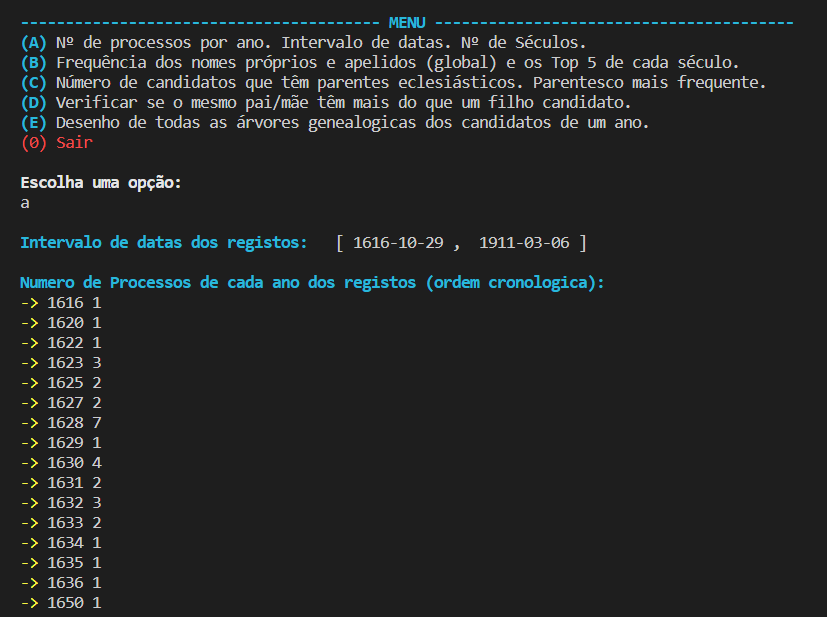
\includegraphics[scale=0.8]{images/a1}
	\captionof{figure}{Resultado da alínea a)}
	\end{center}

	\begin{center}
	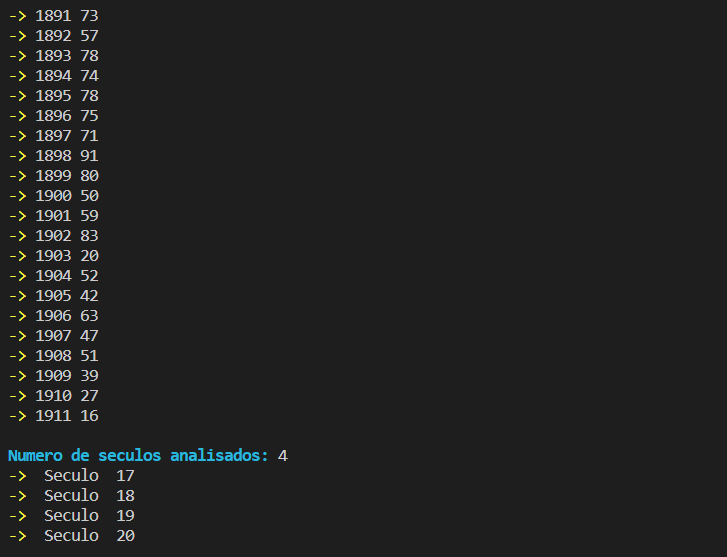
\includegraphics[scale=0.9]{images/a2}
	\captionof{figure}{Resultado da alínea a)}
	\end{center}

\qquad Estes resultados foram verificados através de outros métodos usados como alternativa à solução apresentada. Na figura 4.1 e 4.2 apresentamos apenas um excerto do output relativo ao número de processos de cada ano.
\newpage
\subsection*{ Alínea b)}

\qquad Os resultados obtidos para descobrir os 5 nomes próprios e apelidos mais comuns de cada século foram os seguintes.\par

\begin{center}
	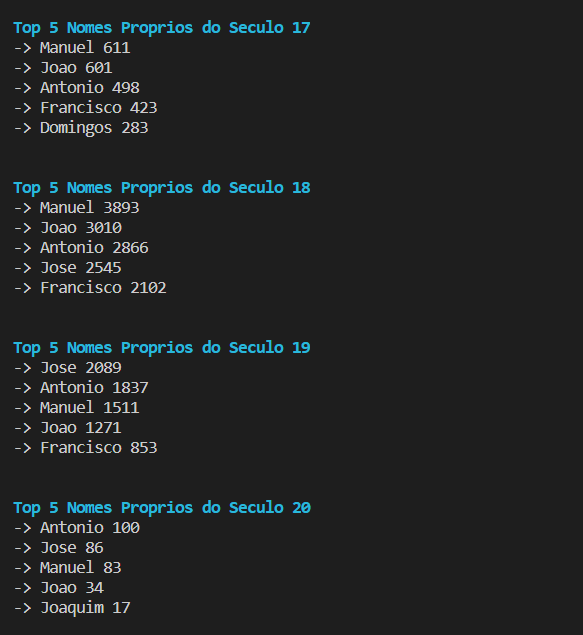
\includegraphics[scale=0.6]{images/b1}
	\captionof{figure}{Resultado da alínea b)}
	\end{center}

\begin{center}
	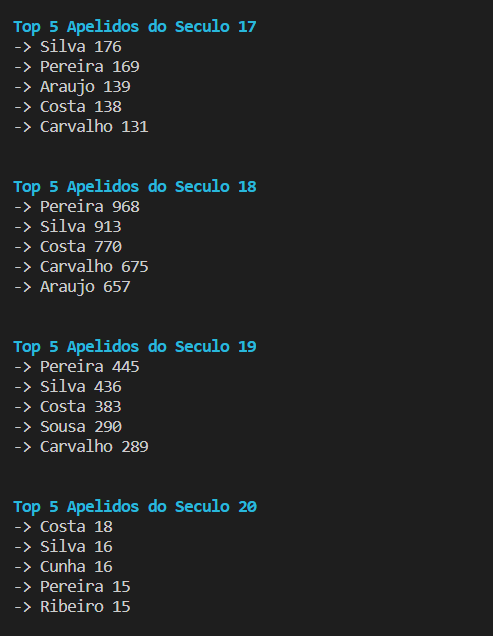
\includegraphics[scale=0.7]{images/b2}
	\captionof{figure}{Resultado da alínea b)}
	\end{center}

\newpage
\qquad Em relação à frequência dos nomes globalmente obtemos o seguinte output: 


\begin{center}
	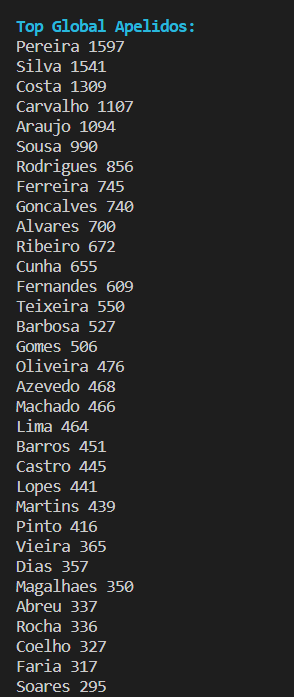
\includegraphics[scale=0.6]{images/b3}
	\captionof{figure}{Resultado da alínea b)}
	\end{center}

\begin{center}
	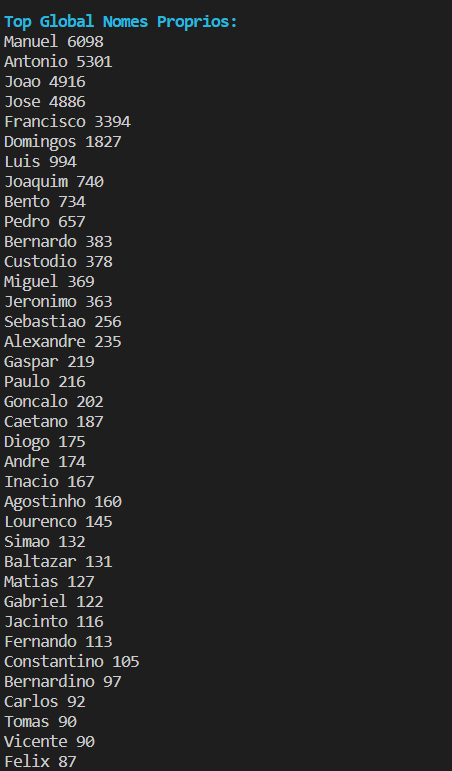
\includegraphics[scale=0.6]{images/b4}
	\captionof{figure}{Resultado da alínea b)}
	\end{center}

\newpage
\subsection*{ Alínea c)}

\begin{center}
	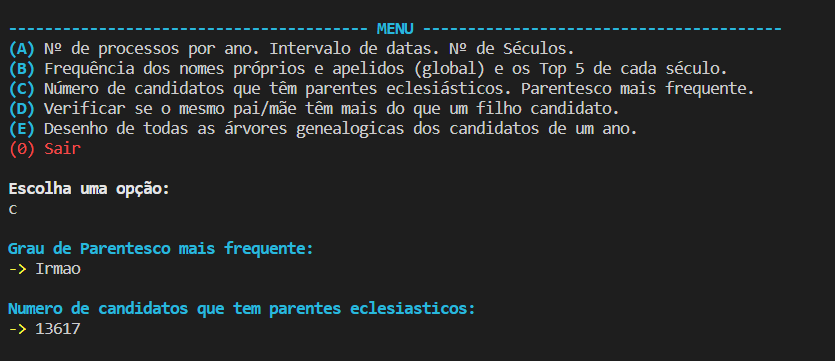
\includegraphics[scale=0.55]{images/c1}
	\captionof{figure}{Resultado da alínea c)}
	\end{center}


\vspace{2.5cm}


\subsection*{ Alínea d)}

\qquad Estes resultados além de apresentarem a resposta ao que é pedido, também indicam qual o id dos processos dos irmãos do candidato.

\begin{center}
	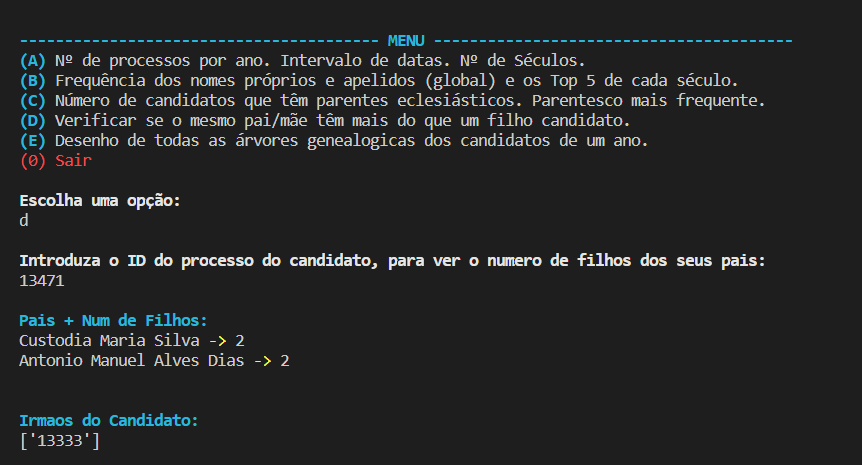
\includegraphics[scale=0.7]{images/d1}
	\captionof{figure}{Resultado da alínea d)}
	\end{center}
\newpage
\subsection*{ Alínea e)}


\qquad Para o seguinte input representado na Figura 4.9, obtemos o resultado da Figura 4.10.

\begin{center}
	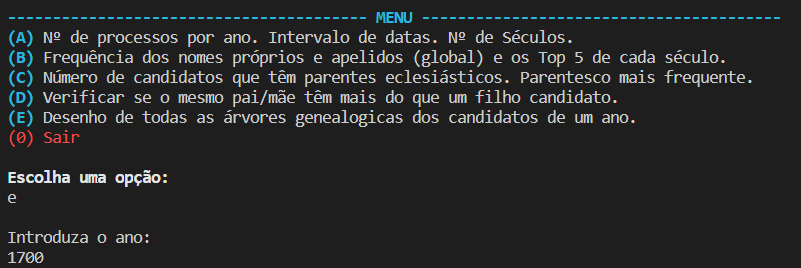
\includegraphics[scale=0.5]{images/e1}
	\captionof{figure}{Input da alínea e)}
	\end{center}


\begin{center}
	
\includegraphics[scale=0.15]{images/e2}
	\captionof{figure}{Resultado da alínea e)}
	\end{center}

\newpage
\section{Problemas e decisões}

\qquad Ao longo da resolução deste trabalho foram encontrados diversos problemas aos quais foram encontradas as devidas soluções. \par
\qquad Em primeiro lugar foi necessário garantir a leitura rápida do ficheiro uma vez que é a parte mais demorada de todos os programas implementados. Assim, para garantir a sua eficiência, foram implementados métodos que percorressem todo o conteúdo do ficheiro textit{XML} apenas uma vez. Aplicando sempre que possível métodos que envolvessem a aplicação das expressões regulares de forma a praticar o conhecimento adquirido através das aulas da UC.\par
\qquad Por outro lado, foram também detetadas incoerências ao nível do ficheiro textit{XML} dado, como por exemplo a existência de pessoas diferentes com o mesmo id ou processos repetidos. Tal como acontece com o \textit{id 21000}, onde existem dois processos distintos com este mesmo número de identificação, para tal foi preciso adaptar o programa e contornar a situação. De qualquer das formas foram considerados processos distintos, apesar do id ser considerado sempre um valor único. 
	  


\section{Alternativas}

\qquad Existem várias alternativas que o grupo poderia ter escolhido para solucionar este problema. Uma delas seria criar um ficheiro próprio para a leitura dos dados de forma a separar a resolução em si da leitura do ficheiro, e, assim, o ficheiro \textit{XML} seria apenas lido, no total, uma só vez. Mas o grupo optou por apresentar uma resolução separada para cada alínea, e um ficheiro global que integra as mesmas.

\chapter{Conclusão} \label{concl}

\qquad A resolução deste projeto permitiu ao grupo consolidar a matéria lecionada ao longo das aulas teóricas e práticas, bem como aprofundar o seu conhecimento em \textit{Python}.\par
\qquad Consideramos que realizamos o trabalho com sucesso, na medida em que respondemos a todos os requisitos pedidos no enunciado, obtendo resultados bastante plausíveis.\par
\qquad Como sugestão para trabalhos futuros, algumas das alíneas poderiam ser feitas de outras formas mais eficientes. 


\appendix % apendice
\chapter{Código do Programa}

\section*{menu.py}

\begin{verbatim}

def print_menu():
    print("\n")
    print("\033[36m\033[1m---------------------------------------- MENU --------------------------------
--------\033[0m")
    print("\033[1m\033[36m(A)\033[0m Nº de processos por ano. Intervalo de datas. Nº de 
Séculos.")
    print("\033[1m\033[36m(B)\033[0m Frequência dos nomes próprios e apelidos (global) e
 os Top 5 de cada século.")
    print("\033[1m\033[36m(C)\033[0m Número de candidatos que têm parentes eclesiásticos.
 Parentesco mais frequente.")
    print("\033[1m\033[36m(D)\033[0m Verificar se o mesmo pai/mãe têm mais do que um filho 
candidato.")
    print("\033[1m\033[36m(E)\033[0m Desenho de todas as árvores genealogicas dos candidatos
 de um ano.")
    print("\033[91m(0) Sair\033[0m")



while(True):
    print_menu()
    print("\n\033[1mEscolha uma opção:\033[0m ")
    op = input()
    op=op.upper()
    if (op=='A'):
        exec(open("a).py").read())
    elif (op=='B'):
        exec(open("b).py").read())
    elif (op == 'C'):
        exec(open("c).py").read())
    elif (op == 'D'):
        exec(open("d).py").read())
    elif (op == 'E'):
        exec(open("e).py").read())
    elif (op=='0'):
        break
    else: print("\033[91m\033[1mOpção inválida.\033[0m")

\end{verbatim}



\section*{a).py}
\begin{verbatim}
import re
from collections import Counter

f = open("processos.xml", "r")

listaAnos = []
listaSeculos = []
listaDatas = []
min = []
max = []
min2 = ''
max2 = ''

for linha in f:
    res = re.search(r'<data>((((\d)|(\d){2})\d{2})(-\d{2}){2})</data>',linha)
    #group(1) -> Data
    #group(2) -> Ano
    #group(3) -> Século - 1

    if (res) :
        listaAnos.append(res.group(2))
        listaSeculos.append(int(res.group(3)) + 1)
        listaDatas.append(res.group(1))
        ''' 
        "work smarter not harder"
        resData = re.split(r'-',res.group(1),0,0)
        if(min== [] and max==[]):
            min=resData
            max=resData
        elif(int(resData[0])> int(max[0])):
            max = resData
        elif(int(resData[0])< int(min[0])):
            min = resData
        elif(int(resData[0])==int(min[0])):
            if(int(resData[1])<int(min[1])):
                min = resData
            elif (int(resData[1])==int(min[1])):
                if(int(resData[2])<int(min[2])):
                    min = resData
        elif (int(resData[0])==int(max[0])):
            if(int(resData[1])>int(max[1])):
                max = resData
            elif (int(resData[1])==int(max[1])):
                if(int(resData[2])>int(max[2])):
                    max = resData

print(min)
print(max) '''

listaAnos.sort()
listaSeculos.sort()


#Solução sem ER para descobrir o intervalo das datas 
listaDatas.sort()
min2 =listaDatas[0]
max2 = listaDatas[len(listaDatas)-1]
print("\n\033[1m\033[36mIntervalo de datas dos registos:\033[0m   [",min2,", ",max2,"]\n")

print("\033[1m\033[36mNumero de Processos de cada ano dos registos (ordem cronologica):\033[0m")

for key, value in (sorted(Counter(listaAnos).items())):
    print("\033[93m->\033[0m", key, value)

i=0
for key in (Counter(listaSeculos).keys()):
    i+=1

print("\n\033[1m\033[36mNumero de seculos analisados:\033[0m", i)
for key in (Counter(listaSeculos).keys()):
    print("\033[93m->\033[0m"," Seculo ", key)




'''
#Solução sem ER para obter os vários séculos
seculos = []
for x in Counter(listaAnos).keys():
    y = (int(x)/100)+1
    seculos.append(int(y))
print(Counter(seculos).keys())

'''
\end{verbatim}

\section*{b).py}
\begin{verbatim}

'''

<nome>([a-zA-Z]+)[a-zA-Z ]* ([a-zA-Z]+)<\/nome>
<nome>([A-Z][a-z]+) ([A-Z][a-z]+ )*([A-Z][a-z]+)<\/nome>

'''

import re
from collections import Counter
from operator import itemgetter
from itertools import groupby

f = open("processos.xml", "r")

listaProprios=[]
listaApelidos=[]
listaSecNomesP=[]
listaSecNomesA=[]
nomeP = ()
nomeA = ()


for linha in f:
    res = re.search(r'<nome>(([A-Z][a-z]+) ([A-Z][a-z]+ )*([A-Z][a-z]+))</nome>',linha)
    # group(1) -> Nome Completo
    # group(2) -> Primeiro Nome
    # group(4) -> Último nome

    res2 = re.search(r'<data>((((\d)|(\d){2})\d{2})-.+)</data>',linha)

    if(res):
        nomeP = res.group(2)
        nomeA = res.group(4)
        listaProprios.append(nomeP)
        listaApelidos.append(nomeA)
    if res2 and nomeP and nomeA:
        seculo = int(res2.group(3))+1
        listaSecNomesP.append((nomeP,seculo))
        listaSecNomesA.append((nomeA,seculo))
        nomeA = ()
        nomeP = ()


listaSecNomesP = sorted(listaSecNomesP, key=lambda x: x[1])
X1 = [list(group) for key, group in groupby(listaSecNomesP, itemgetter(1))]

listaSecNomesA = sorted(listaSecNomesA,  key=lambda x: x[1])
X2 = [list(group) for key, group in groupby(listaSecNomesA, itemgetter(1))]


words = Counter(listaProprios).most_common()
print("\n\033[1m\033[36mTop Global Nomes Proprios:\033[0m ")
for key, value in words:
    print(key, value)

words2 = Counter(listaApelidos).most_common()
print("\n\033[1m\033[36mTop Global Apelidos:\033[0m ")
for key, value in words2:
    print(key, value)
print("\n")


for i in X1:
    seculo = i[0][1]
    print("\033[1m\033[36mTop 5 Nomes Proprios do Seculo" , seculo ,"\033[0m" )
    for key, value in (Counter(i).most_common(5)):
        print("->",key[0], value)
    print("\n")

for i in X2:
    seculo = i[0][1]
    print("\033[1m\033[36mTop 5 Apelidos do Seculo" , seculo ,"\033[0m" )
    for key, value in (Counter(i).most_common(5)):
        print("->",key[0], value)
    print("\n")



\end{verbatim}


\section*{c).py}
\begin{verbatim}

import re
from collections import Counter

f = open("processos.xml", "r")
content = f.read()
contador = 0
listaP = []


observacoes = re.findall(r'(<obs>(\n|.)*?</obs>)', content)
for obs in observacoes:
    res2 = re.findall(r'(Irmao|Tio|Primo)', obs[0])

    if (res2):
        contador+=1
        for x in res2:
            listaP.append(x)

parFreq = (Counter(listaP).most_common(1))

print("\n\033[36m\033[1mGrau de Parentesco mais frequente:\033[0m ")
for key, value in parFreq:
    print("\033[93m->\033[0m",key)

print("\n\033[36m\033[1mNumero de candidatos que tem parentes eclesiasticos:\033[0m ")
print("\033[93m->\033[0m", contador)

\end{verbatim}


\section*{d).py}
\begin{verbatim}

import re
import sys
from collections import Counter

f = open("processos.xml", "r")

content = f.read()
print("\n\033[1mIntroduza o ID do processo do candidato, para ver o numero de filhos
 dos seus pais:\033[0m ")
filho = input()
irmaos = []
pais=[] #pais[0] = mãe; pais[1] = pai
traicoes=[]

def procuraID(id,filho1):
    m = re.search(rf'<processo id="({id})">(\n|.)*?</processo>', content)
    if (m):
        processo = m.group()
        rmae = re.search(r'<mae>(([A-Z][a-z]+) ?([A-Z][a-z]+ )*([A-Z][a-z]+)?).*</mae>',processo)
        rpai = re.search(r'<pai>(([A-Z][a-z]+) ([A-Z][a-z]+ )*([A-Z][a-z]+)).*</pai>',processo)
        if(rmae):
            mae = rmae.group(1)
        else:
            mae = '' #caso não tenha mãe
        if(rpai):
            pai = rpai.group(1)
        else:
            pai = '' #caso não tenha pai

        if(filho1 == 1): # é o 1º filho que procuramos, corresponde ao ID que o User fornece
            pais.append(mae)
            pais.append(pai)
            if re.search(r'<obs>', processo):
                res2 = re.findall(r'(Irmao). *Proc.(\d+)',processo)
                if(res2):
                    for x in res2:
                        irmaos.append(x[1])

        elif (filho1 == 0):  # é irmão

            if (mae == pais[0]):
                pais.append(mae)
            else:
                traicoes.append(pai) #caso o irmão tenha mãe diferente de um dos irmãos

            if (pai == pais[1]):
                pais.append(pai) 
            else:
                traicoes.append(mae) #caso o irmão tenha pai diferente de um dos irmãos

'''
# Teste com todos os ids, verificando traições entre casais
lista = re.findall(rf'<processo id="(\d+)">',content)
for i in lista:
    print(i)
    procuraID(i,1)
    for x in irmaos:
        procuraID(x, 0)
    #print(Counter(pais))
    #print(irmaos)
    print("Traicoes: ",traicoes)
    pais=[]
    irmaos=[]
'''
procuraID(filho,1)
for i in irmaos:
    procuraID(i,0)

paisRes = Counter(pais).most_common()
print("\n\033[36m\033[1mPais + Num de Filhos:\033[0m")
for key, value in paisRes:
    print(key,"\033[93m->\033[0m", value)

print("\n")
print("\033[36m\033[1mIrmaos do Candidato:\033[0m ")
print(irmaos)


#21000 -> processo distinto com o ID repetido


\end{verbatim}


\section*{e).py}
\begin{verbatim}

import re
from collections import Counter
from graphviz import Digraph

f = open("processos.xml", "r")
content = f.read()
i = 0
lista = []

def procuraIrmao(id,lista):
    for i in lista:
        processo = i[0]
        m = re.search(rf'<processo id="({id})">', processo)
        if (m):
            rnome = re.search(r'<nome>(([A-Z][a-z]+) ?([A-Z][a-z]+ )*([A-Z][a-z]+)?).*</nome>',
		 processo)
            if(rnome):
                nome = rnome.group(1)
                lista.remove(i)
                return nome
    return False

def desenhaFamilias(familia,dot,i):
    mae = str(i)
    pai = str(i+1)
    dot.node(mae, familia[1])   #mae
    dot.node(pai, familia[2])   #pai
    dot.node(str(i+2), familia[0])   #filho

    dot.edge(mae, str(i+2))
    dot.edge(pai, str(i+2))
    i = i+3
    if len(familia) > 3:
        for x in range(3,len(familia)):
            dot.node(str(i), familia[x])
            dot.edge(mae, str(i))
            dot.edge(pai, str(i))

    #print(dot.source)
    return (dot,i)


def processosAno(ano):
    treeFam = []
    lista = re.findall(rf'(<processo id="(\d+)">\n *<pasta>\d+</pasta>\n *
		<data>({ano})-.+(\n|.)*?</processo>)', content)
    for i in lista:
        familia = []
        processo = i[0]
        rfilho = re.search(r'<nome>(([A-Z][a-z]+) ?([A-Z][a-z]+ )*([A-Z][a-z]+)?).*</nome>',
		 processo)
        rmae = re.search(r'<mae>(([A-Z][a-z]+) ?([A-Z][a-z]+ )*([A-Z][a-z]+)?).*</mae>',
		 processo)
        rpai = re.search(r'<pai>(([A-Z][a-z]+) ([A-Z][a-z]+ )*([A-Z][a-z]+)).*</pai>',
		 processo)
        if (rmae):
            mae = rmae.group(1)
        else:
            mae = False  # caso não tenha mãe
        if (rpai):
            pai = rpai.group(1)
        else:
            pai = False  # caso não tenha pai
        if (rfilho):
            filho = rfilho.group(1)
            familia.append(filho)
            familia.append(mae)
            familia.append(pai)
        if re.search(r'<obs>', processo):
            res2 = re.findall(r'(Irmao). *Proc.(\d+)', processo)
            if (res2):
                for x in res2:
                    irmao = procuraIrmao(x[1],lista)
                    if irmao !=False:
                        familia.append(irmao)

        treeFam.append(familia)
    return treeFam



print("\nIntroduza o ano: ")
ano = input()
treeFam = processosAno(ano)
dot = Digraph(comment=f'Arvore Genealogica dos Candidatos do Ano {ano}', engine = 'neato',
	 format='png')

for familia in treeFam:
    print(familia)
    (dot,i) = desenhaFamilias(familia,dot,i)
    i=i+1

dot.render(f'test-output/arvoreGenealogica{ano}.gv', view=True)

\end{verbatim}

\end{document} 